%%% PREAMBLE - Do not touch %%%%%%%%%%%%%%%%%%%%%%%%%%%%%%%%%%%%%%%%%%%%%%%%%%%%%%
\documentclass[10pt,twocolumn,letterpaper]{article}
\usepackage[ansinew]{inputenc}
\usepackage[portuges,brazil,english]{babel}
\usepackage{model}
\usepackage{times}
\usepackage{epsfig}
\usepackage{graphicx}
\usepackage{amsmath}
\usepackage{amssymb}
\usepackage{color}
\usepackage[pagebackref=true,breaklinks=true,letterpaper=true,colorlinks,bookmarks=false]{hyperref}

\usepackage{float}
\usepackage{graphicx}
\usepackage{wrapfig}
\usepackage{algpseudocode,algorithm}
\usepackage{listings}

\lstset{ %
  backgroundcolor=\color{white},   % choose the background color; you must add \usepackage{color} or \usepackage{xcolor}
  basicstyle=\footnotesize,        % the size of the fonts that are used for the code
  breakatwhitespace=false,         % sets if automatic breaks should only happen at whitespace
  breaklines=true,                 % sets automatic line breaking
  commentstyle=\color{gray},    % comment style
  deletekeywords={...},            % if you want to delete keywords from the given language
  escapeinside={\%*}{*)},          % if you want to add LaTeX within your code
  extendedchars=true,              % lets you use non-ASCII characters; for 8-bits encodings only, does not work with UTF-8
  frame=single,                    % adds a frame around the code
  keepspaces=true,                 % keeps spaces in text, useful for keeping indentation of code (possibly needs columns=flexible)
  keywordstyle=\color{blue},       % keyword style
  language=Python,                 % the language of the code
  numbers=left,                    % where to put the line-numbers; possible values are (none, left, right)
  numbersep=5pt,                   % how far the line-numbers are from the code
  numberstyle=\tiny\color{gray},   % the style that is used for the line-numbers
  rulecolor=\color{black},         % if not set, the frame-color may be changed on line-breaks within not-black text (e.g. comments (green here))
  showspaces=false,                % show spaces everywhere adding particular underscores; it overrides 'showstringspaces'
  showstringspaces=false,          % underline spaces within strings only
  showtabs=false,                  % show tabs within strings adding particular underscores
  stepnumber=2,                    % the step between two line-numbers. If it's 1, each line will be numbered
  stringstyle=\color{red},         % string literal style
  tabsize=2,                       % sets default tabsize to 2 spaces
  title=\lstname                   % show the filename of files included with
 }

\pagenumbering{gobble}

\cvprfinalcopy
\def\httilde{\mbox{\tt\raisebox{-.5ex}{\symbol{126}}}}
\ifcvprfinal\pagestyle{empty}\fi

\newcommand{\TODO}[1]{TODO: #1}
\newcommand{\CITEONE}[2]{\mbox{#1 \cite{#2}}}
\newcommand{\CITETWO}[3]{\mbox{#1 and #2 \cite{#3}}}
\newcommand{\CITEN}[2]{\mbox{#1 et al. \cite{#2}}}

%%% Report beginning %%%%%%%%%%%%%%%%%%%%%%%%%%%%%%%%%%%%%%%%%%%%%%%%%%%%%%%%%%%%%
\begin{document}

%%% Title and authors %%%%%%%%%%%%%%%%%%%%%%%%%%%%%%%%%%%%%%%%%%%%%%%%%%%%%%%%%%%%
\title{A Multi-Layer Modeling Approach to Music Genre Classification}
\author{Renan V. Novas
%		\thanks{\textbf{Contact}:\tt\small{}} \\
		\\
		Gabriel S. Vicente
		\thanks{\textbf{Contact}: \tt\small{ra116953@ime.unicamp.br}} }

\maketitle
%%% Abstract %%%%%%%%%%%%%%%%%%%%%%%%%%%%%%%%%%%%%%%%%%%%%%%%%%%%%%%%%%%%%%%%%%%%%
\begin{abstract}
Listening to music and understanding its patterns and structure is
a fairly easy task for humans beings, even for listeners without formal musical education.
However, building computational models to mimic those processes has proven a
remarkably resilient problem. The algorithms and data associated to the Music
Information Retrieval (MIR) field are both complex.

The scientific endeavour is motivated by a large class of challenging demands in
the media business that require efficient and robust audio classification.
Application scenarios include audio streaming services, such as Spotify and
Pandora, automatic media monitoring, content-based search in multimedia
databases, improvements on recommendation and filtering systems and last, but
not least, purely artistic explorations.
\end{abstract}
%%% Introduction %%%%%%%%%%%%%%%%%%%%%%%%%%%%%%%%%%%%%%%%%%%%%%%%%%%%%%%%%%%%%%%%%
\section{Motivation}

Musical genre is notoriously subjective concept and its classification has been
a standard problem in the Musical Information Retrieval (MIR) research. It is
a very active and multidisciplinary investigation field, comprising musicology,
psychology, signal processing, artifial intelligence and machine learning. MIR
applications can be divided typically in four groups.

\begin{itemize}
  \item Instrument and musical structure recognition
  \item Recommendation and taste prediction engines
  \item Automatic music transcription and algorithmic composition 
  \item Automatic categorization
\end{itemize}

We are here interested in the last. An extraordinary range of information is
hidden inside of music waveforms, ranging from perceptual to auditory which
inevitably makes large-scale applications challenging. There are a number of commercially successful online music services, 
such as Spotify, Pandora and Last.fm, but most of them are merely
based on traditional text information retrieval. Many different features can be
used for music classification, such as reference features including title and
composer, content-based acoustic features including tonality, pitch, and beat,
symbolic features extracted from the scores. Content-based music genre classification has been gaining importance and enjoying a growing amount of
attention. Commonly used classifiers
include Support Vector Machines (SVMs), Nearest-Neighbor (NN) classifiers, Gausian Mixture Models and Linear Discriminant Analysis (LDA).

%%% Add section %%%%%%%%%%%%%%%%%%%%%%%%%%%%%%%%%%%%%%%%%%%%%%%%%%%%%%%%%%%%%%%%%%
\section{Related Work}

A long line of work addresses problems in the Music Information Retrieval. There
are a growing interest in the scientic community and a vast diversity of new
content-based models \cite{conf/sigir/HuO12} \cite{Bou-rabee12classifyingthe}.
The content-based acoustic features are classified into timbral texture features, rhythmic content features and pitch content
features. Timbral features are mostly originated from traditional speech
recognition techniques. They are usually calculated for every short-time frame
of sound based on the Short Time Fourier Transform (STFT) and countless others
audio descriptos, such as Mel-Frequency Cepstral Coefficients (MFCCs). More
atypical descriptors, such as Daubechies Wavelet
Coefficient Histograms (DWCH), have been used in experimentation
\cite{Li:2003:CSC:860435.860487}.
%%% Add section %%%%%%%%%%%%%%%%%%%%%%%%%%%%%%%%%%%%%%%%%%%%%%%%%%%%%%%%%%%%%%%%%%
\section{Experiments and Discussion}

We used several approaches to leverage different types of information about a
song into a final classifier. First of all, we look in more detail to dataset.

\subsection{Million Song Dataset}

The Million Song Dataset (MSD) \cite{Bertin-Mahieux2011} is a freely-available
collection of audio features and metadata for a million contemporary popular
music tracks. The project emerged as a collaborative enterprise between The
Echo Nest (now a subsidiary of Spotify) and Columbia University's
Laboratory for the Recognition and Organization of Speech and Audio (LabROSA) to
provide a dataset collection for evaluating audio-related research and to
encourage algorithms that scale to commercial sizes.

\begin{wrapfigure}{R}{0.10\textwidth}
\centering
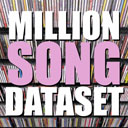
\includegraphics[width=0.1\textwidth]{img/LogoMSD.jpg}

\includegraphics[width=0.1\textwidth]{img/LogoTheEchoNest.jpg}

\includegraphics[width=0.1\textwidth]{img/LogoLabROSA.jpg}
\end{wrapfigure} 

The dataset itself does not include any audio signal, only derived
features. It constains nearly $300$ GB of metadata and audio-descriptive
data, available as an Amazon Public Dataset (AWS), or through a
directly-downloadable subset consisting of $10,000$ songs selected at random for
a quick look. 

\begin{itemize}
  \item \textbf{Million Song Dataset}
  \begin{itemize}
  \item 280 GB of data
  \item 1,000,000 songs/files
  \item 44,745 unique artists
  \item 7,643 The Echo Nest tags 
  \item 2,321 MusicBrainz tags
  \item 2,201,916 asymmetric similarity relationships
  \item 515,576 dated tracks starting from 1922
  \end{itemize}
\end{itemize}

Each audio track is
associated to an exclusive Echo Nest song ID, to artist and song metadata and
to numerical fields taken directly from the Echo Nest Analyze API. It is indeed
a very extensive and scalable dataset. 
 
However, the dataset involved in this present experiment is  modest
comparing to the MSD. Since the original collection does not
explicitly provide genre information, we recreated a smaller dataset while using 
additional databases. The idea is to use
artist tags that describe typical artist-genre associations to assign the
information to each track. We used MusicBrainz \cite{MusicBrainz} tags instead
of hand-picking associations as they were applied by humans and usually very reliable. They also
tend to be standardized, as MusicBrainz care for consistency. We applied the routine to a subset, yielding
$16,00$ different tracks, of which 90\% were selected at random for training.

\begin{table}[H]
\begin{center}
\caption{List of genres groups and number of sample tracks}
\begin{tabular}{|l|l|c|c|}
\hline
&\textbf{Genre}   	    & Training & Test    \\ \hline
A&dance and electronica & 2,880 	 & 320   \\
B&folk           		& 2,880	     & 320	 \\
C&jazz and blues        & 2,880 	 & 320   \\
D&punk				    & 2,880      & 320   \\
E&soul and reggae       & 2,880	     & 320   \\ \hline
 &					    & 14,400	 & 1,600 \\ \hline
\end{tabular}
\end{center}
\end{table}

Evidently, building such simplified dataset implies huge flaws. The main one is the unbalancedness of the data. In
our case, we selected the same cardinality of songs to each group. A more subtle
issue is the genre definition itself. Music genre is notoriously subjective
concept. Indicating genre is far more complex than a trivial binary
classification and often inconclusive and appropriate to ambiguity.
We considered only artists that have been tagged consistenty. We could argue the
label of a particular track, but they were still reasonable. It is a little
extreme, but we wanted to avoid confusing artists, such as those that span more
than one genre.

\subsection{Audio features}

As for audio features, timbre is represented as 12-dimensional vectors that are
the principal components of Mel-frequency cepstral coefficients (MFCCs); they represent the power spectrum of sound, and are derived from
Fourier analysis and further processing. MFCCs are very commonly used in speech
recognition and music information retrieval systems. Also track level audio
features such as loudness and tempo which captures the high level information of the audio. T
empo is defined as number of beats per minute, or BPM and loudness is a real value number describes the general loudness of the song.

So use the simplest 30 audio features from The Echo Nest: loudness,
tempo, time signature, key, mode, duration, 12 averages and 12 variances of timbre
vectors. 

\subsection{Results and Analysis}

We experimented at first a multi-class classification using 15 different support
vector machines (SVMs) from the open-source Python implementation
of the \texttt{Scikit-learn} project \cite{scikit-learn}. More detailed
information is avaiable in the documentation. We set up kernel
parameter to \textcolor{red}{rbf}, C to \textcolor{red}{1} and gamma to
\textcolor{red}{0}. The following code matrix served as input. \emph{One-vs-One} correponds to 1-10 models and \emph{One-vs-Rest} to 11-15.
For those models, we mutiplied C by weights inversely proportional to the frequency of each SVM classes, in order to perform some balancing.

\begin{table}[H]
\begin{center}
\caption{Code Matrix}
\begin{tabular}{|l|*5{c|}}
\hline
\textbf{SVM}& A & B & C & D & E \\ \hline
1& 1 & -1& 0 & 0 & 0 \\ \hline
2& 1 & 0 & -1& 0 & 0 \\ \hline
3& 1 & 0 & 0 & -1& 0 \\ \hline
4& 1 & 0 & 0 & 0 & -1 \\ \hline
5& 0 & 1 & -1& 0 & 0 \\ \hline
6& 0 & 1 & 0 & -1& 0 \\ \hline
7& 0 & 1 & 0 & 0 & -1 \\ \hline
8& 0 & 0 & 1 & -1&  0 \\ \hline
9& 0 & 0 & 1 & 0 & -1 \\ \hline
10& 0 & 0 & 0 & 1 & -1 \\ \hline
11& 1 & -1& -1& -1& -1 \\ \hline
12& -1& 1 & -1& -1& -1 \\ \hline
13& -1& -1&  1& -1& -1 \\ \hline
14& -1& -1& -1&  1& -1 \\ \hline
15& -1& -1& -1& -1&  1 \\ \hline
\end{tabular}
\end{center}
\end{table}

For each model, we considered 80\% of random samples for 
training and 20\% for a \emph{leave-one-out} validation. All informations, in
training, validation and test, were normalized using the mean values and
stardard deviations of corresponding model.

\begin{table}[H]
\begin{center}
\caption{Scores}
\begin{tabular}{|l|*2{c|}}
\hline
 				& \multicolumn{2}{c|}{Normalized Accuracies} \\ \hline
 				
\textbf{SVM}	& Training  & Validation \\ \hline
1				& 92.5\% 	& 87.2\%	 \\ 
2				& 88.4\%	& 83.5\%	 \\ 	
3				& 91.2\%	& 86.9\%	 \\ 
4				& 93.7\%	& 90.7\%	 \\ 
5				& 89.8\%	& 83.9\%	 \\ 
6				& 87.6\%	& 83.2\%	 \\ 
7				& 90.6\%	& 87.2\%	 \\
8				& 90.1\%	& 86.3\%	 \\ 
9				& 93.5\%	& 90.4\%	 \\ 
10				& 91.9\%	& 86.9\%	 \\ 
11				& 86.7\%	& 84.2\%	 \\ 
12				& 88.1\%	& 84.7\%	 \\ 
13				& 87.7\%	& 85.0\%	 \\ 
14				& 84.3\%	& 80.9\%	 \\ 
15 				& 91.8\%	& 88.5\%	 \\ \hline
\end{tabular}
\end{center}
\end{table}

\subsection{A Multi-Layer Approach}

Our first innocent attack has given us 15 differents classifiers. We offered
them our initial dataframes, expecting predictions we
may now attach as features to a more complex 2-layer model. We devised a
\emph{Extremely Randomized Trees} \cite{Geurts} approach, also
implemented in \texttt{Scikit-learn} packages. We employed the \emph{bagging} algorithm for constructing forest trees
and \emph{out-of-the-bag} for scoring success rate. Futhermore, in order to
optimize the forest constructing parameters, we performed grid search. The best
setting was \textcolor{red}{90} trees, \textcolor{red}{6} features at maximum
and \textcolor{red}{3} samples for leaf at minimum. 

\begin{table}[H]
\begin{center}
\caption{Confusion Matrix}
\begin{tabular}{|l|*5{c|r|}}
\hline
 & \multicolumn{5}{c|}{Predicted Genre} & \\ \hline
 & A  & B  & C  & D  & E  &     \\ \hline
A& 224& 21 & 24 & 17 & 34 & 320 \\ \hline
B& 12 & 224& 39 & 15 & 30 & 320 \\ \hline
C& 27 & 42 & 223&  9 & 19 & 320 \\ \hline
D& 24 & 15 & 7  &240 & 34 & 320 \\ \hline
E& 39 & 36 & 16 & 11 & 218& 320 \\ \hline
 & 326 &338 & 309 & 292 & 335 & \\ \hline
\end{tabular}
\end{center}
\end{table}

The average impact of SVM-related features was approximately 0.8\%, with at most
7.46\% of contribution. In fact, the original 30 features remained the most
relevant. The success rate of 86.99\% was attained in
training and 76.9\% in an \emph{out-of-the-bag} scenario. In test, we
accomplished 70.56\% rate of successfully categorized songs. We
achieved 70.56\% of sucessfully categorizing tracks in the test dataset.
Comparatively, more usual random forest models yields 69\%-70\%.

\subsection{Alternative Solutions}

In our experiments, we extended the test to several initial procedures. Using
exclusively the SVM-related features, our best results were a single
\emph{random forest} \cite{Breiman} with 150 trees and 150 at maximum leaf nodes. The
success rate reached 79.19\% in training, 77.15\% \emph{out-of-the-bag} and
69.13\% in test. \emph{One-vs-One} models contributed with nearly 4\%, while
\emph{One-vs-Rest} models were more important, holding 10\%. 

Using the original 30 features, the best result was again a \emph{random forest}
with 450 tress. Obtaining success on 70.79\% of the training cases, 68.64\%
\emph{out-of-the-bag} and 68.64\% in test.

Comparing the three models in order of appearance: \\

\begin{figure}[H]
\centering
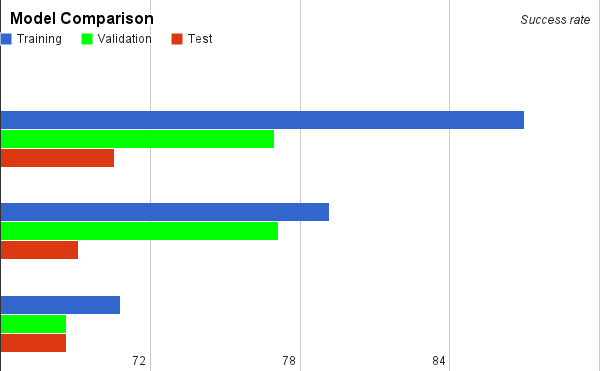
\includegraphics[width=0.4\textwidth]{img/ModelComparison.png}
\end{figure}

Exploring further, multi-class classifiers such as ECOC, \emph{One-vs-One},
\emph{One-vs-Rest} without proper tuning do not yield impacting results, ranging
from 35\% to 40\% success rate in test.
%%% Add section %%%%%%%%%%%%%%%%%%%%%%%%%%%%%%%%%%%%%%%%%%%%%%%%%%%%%%%%%%%%%%%%%%
\section{Conclusions and Future Work}
In this project, we proposed a multi-layer modeling approach to music genre
classification. The \emph{Extremely Randomized Tree} model showed
the best results, using SVM classfiers for feature extraction. We accomplished
70.56\% of success rate in test. Looking at the confusion matrix, it is evident
we avoided bias.
Since genre tags were associated to artists in our experiment, musical
compositions considerably different from the artist's usual characteristics and
patters might explain some of the confusion. In the future, it would be interesting analysing
cases in which the final classification is a more valid answer than our target
valu
Considering hypothetically the similiary matrices indicate stable results, it
would possible to imply that some tracks are wrongly classified because its
artist cannot be exclusively assigned to a particular genre. In the future, it
would be convenient to analyse overlapping and ambiguity.


%%% References %%%%%%%%%%%%%%%%%%%%%%%%%%%%%%%%%%%%%%%%%%%%%%%%%%%%%%%%%%%%%%%%%%%
{\small
\bibliographystyle{unsrt}
\bibliography{refs}
}

%\onecolumn
%\section*{Source Code}
%\lstinputlisting[caption=Filtering And Sampling,language=Python]
%{../../Codes/Usados/FilteringAndSampling.py} 

%\lstinputlisting[caption=Auxiliary Functions,language=Python]
%{../../Codes/Usados/header.py}

%\lstinputlisting[caption= Classification,language=Python]
%{../../Codes/Usados/ecocSVM.py}

\end{document}